\section{Introduction}
% Learning latent dynamics models from high-dimensional observations such as images is a promising avenue toward letting our artificial and physical agents better and efficiently understand the world around them and is essential for achieving both artificial and physical intelligence~\cite{}
Learning how the environment evolves around us from high-dimensional observations (i.e., world models~\cite{ha2018world}) is essential for achieving both artificial and physical intelligence~\cite{hafner2023mastering}.
For example, world models are required for effectively planning an artificial/robotic agent's actions in complex and unstructured environments~\cite{matsuo2022deep}. 
However, learning such dynamics directly in high-dimensional observation space is usually intractable. Seminal works have shown that we can leverage autoencoders to compress the state information into a low-dimensional latent space~\cite{liou2014autoencoder, kingma2014auto} in which it is much more feasible to learn the dynamics~\cite{watter2015embed, lenz2015deepmpc, wahlstrom2015learning, champion2019data, zhong2020unsupervised}.
%
However, strong limitations still persist when it comes to using these learned models to generate low-level intelligence.

One outstanding challenge is how to perform closed-loop control in the learned latent space - i.e., how to generate control inputs based on a high dimensional sensory input such that a desired movement is generated. Prior works have explored, among other approaches, \gls{RL}~\cite{van2016stable, gelada2019deepmdp, hafner2019dream, schwarting2021deep}, \gls{MPC}~\cite{lenz2015deepmpc, hafner2019learning, hewing2020learning, alora2023robust}, \glspl{LQR}~\cite{brunton2016koopman, mamakoukas2019local, haggerty2023control} and gradient-based optimization~\cite{yamada2023leveraging} for planning and control towards a target evolution that is given in observation space.
However, all existing latent-space control strategies have shortcomings, such as a limited planning horizon and slow control rates (\gls{MPC} and gradient-based approaches), sample inefficiency (RL), or they pose a requirement for learning linear dynamics~\cite{watter2015embed} (\gls{LQR}), which is not even possible for systems that are inherently non-linearizable~\cite{cenedese2022data}.
One interesting avenue is to leverage model-based control approaches, such as potential shaping~\cite{bloch2001controlled, ortega2021pid, zhong2020unsupervised}, for effective and computationally efficient control in latent space~\cite{lepri2023neural}. 
For these techniques to be feasible, the dynamical model needs to fulfill four characteristics: (i) the dynamics need to have the mathematical structure of physical systems, (ii) conserve the stability properties of real systems, (iii) the latent state needs to be relatively low-dimensional, and (iv) there needs to exist a well-defined, invertible mapping between the input and the forcing in latent space.
% the latent state needs to be relatively low-dimensional, (3) there needs to exist a well-defined, invertible mapping between the input and the forcing in latent space, and (4) the latent dynamics need to be easily stabilizable.
However, existing model structures that are used for learning latent dynamics~\cite{botev2021priors} do not meet all of these criteria. Relevant examples are \glspl{MLP}, \glspl{NODE}~\cite{chen2018neural, sholokhov2023physics}, many variants of \glspl{RNN} (e.g., LSTMs~\cite{hochreiter1997long}, \glspl{GRU}~\cite{cho2014learning}, etc.), and physics-informed neural networks (e.g., \glspl{LNN}~\cite{lutter2018deep, cranmer2020lagrangian, zhong2020unsupervised}, \glspl{HNN}~\cite{greydanus2019hamiltonian}). For example, \glspl{MLP} do not have a physical interpretation and do not provide an invertible mapping of the forcing generated by the input, \glspl{NODE} are usually not easily stabilizable~\cite{white2023stabilized}, most \glspl{RNN} require a relatively high-dimensional latent space (i.e., many hidden states), and energy-shaping control approaches based on \glspl{LNN}~\cite{zhong2020unsupervised} do not come with any formal stability guarantees. %Interestingly, \glspl{LNN} and HNNs could be a valid venue, are empirically %\glspl{LNN} are often not stabilizable when trained in latent-space.

In recent years, oscillatory networks~\cite{rusch2020coupled, rusch2021unicornn, ceni2024random, lanthaler2024neural, rusch2024oscillatory} have been shown to exhibit state-of-the-art performance on time sequence modeling tasks while being parameter-efficient, thus fulfilling our requirement (iii).
% As we have a good understanding of the behavior of harmonic oscillators, they are also interpretable.
%
Consequently, we believe that they are a promising option for control-oriented dynamics learning in latent space.
%
Still, these models do not fulfill the remaining requirements that we have listed above. % open gaps (i),(ii), and (iv). 
%
Despite being an interpretable combination of harmonic oscillators, they do not have the structure of a physical system - i.e., they do not possess a well-defined energy function.
%
Moreover, only local stability~\cite{rusch2020coupled, ceni2024random} has been shown, with sufficient conditions that appear to be very stringent. %, as the energy dissipation of these networks cannot be modeled.
%
Finally, in addition to training an encoder that maps inputs to latent-space forcing, we propose also training a decoder that learns to reconstruct inputs based on latent-space forcing. This enables us to easily switch between inputs and forcing, which is essential when implementing control strategies.

We resolve all the above-mentioned challenges by proposing \glspl{CON}, a new formulation of a coupled oscillator network that is inherently \gls{ISS} stable, for learning the dynamics of physical systems and subsequently exploiting its structure for model-based control in latent space.
The network consists of damped, harmonic oscillators connected through elastic springs, damping elements, and a neuron-like coupling force and can be excited by a nonlinear actuation term.
We identify a transformation into a set of coordinates from which we can derive the networks' kinetic and potential energy.
This allows us to leverage Lyapunov arguments~\cite{khalil2002nonlinear} for proving the global asymptotic stability of the unforced system and \gls{ISS} stability for the forced system under relatively mild assumptions on the network parameters.
Even though we constrain the dynamics to a very specific structure, we demonstrate (a) the CON network achieves similar performance as \glspl{NODE} when learning the dynamics of unactuated, mechanical systems with two orders of magnitude fewer parameters and (b) that the proposed model achieves, for the complex task of learning the actuated, highly nonlinear dynamics of continuum soft robots~\cite{alora2023data, stolzle2021piston} directly from pixels, a \SI{60}{\percent} lower prediction error than \gls{coRNN}~\cite{rusch2020coupled} and reaches the SoA performance across all techniques that we tested.
Finally, we show some initial results that the proposed \gls{CON} model is also able to learn the latent dynamics of \glspl{PDE}, in this case containing reaction-diffusion~\cite{champion2019data, epstein2016reaction} dynamics.

\begin{figure}[t]
    \centering
    \subfigure[Coupled Oscillator Network (CON)]{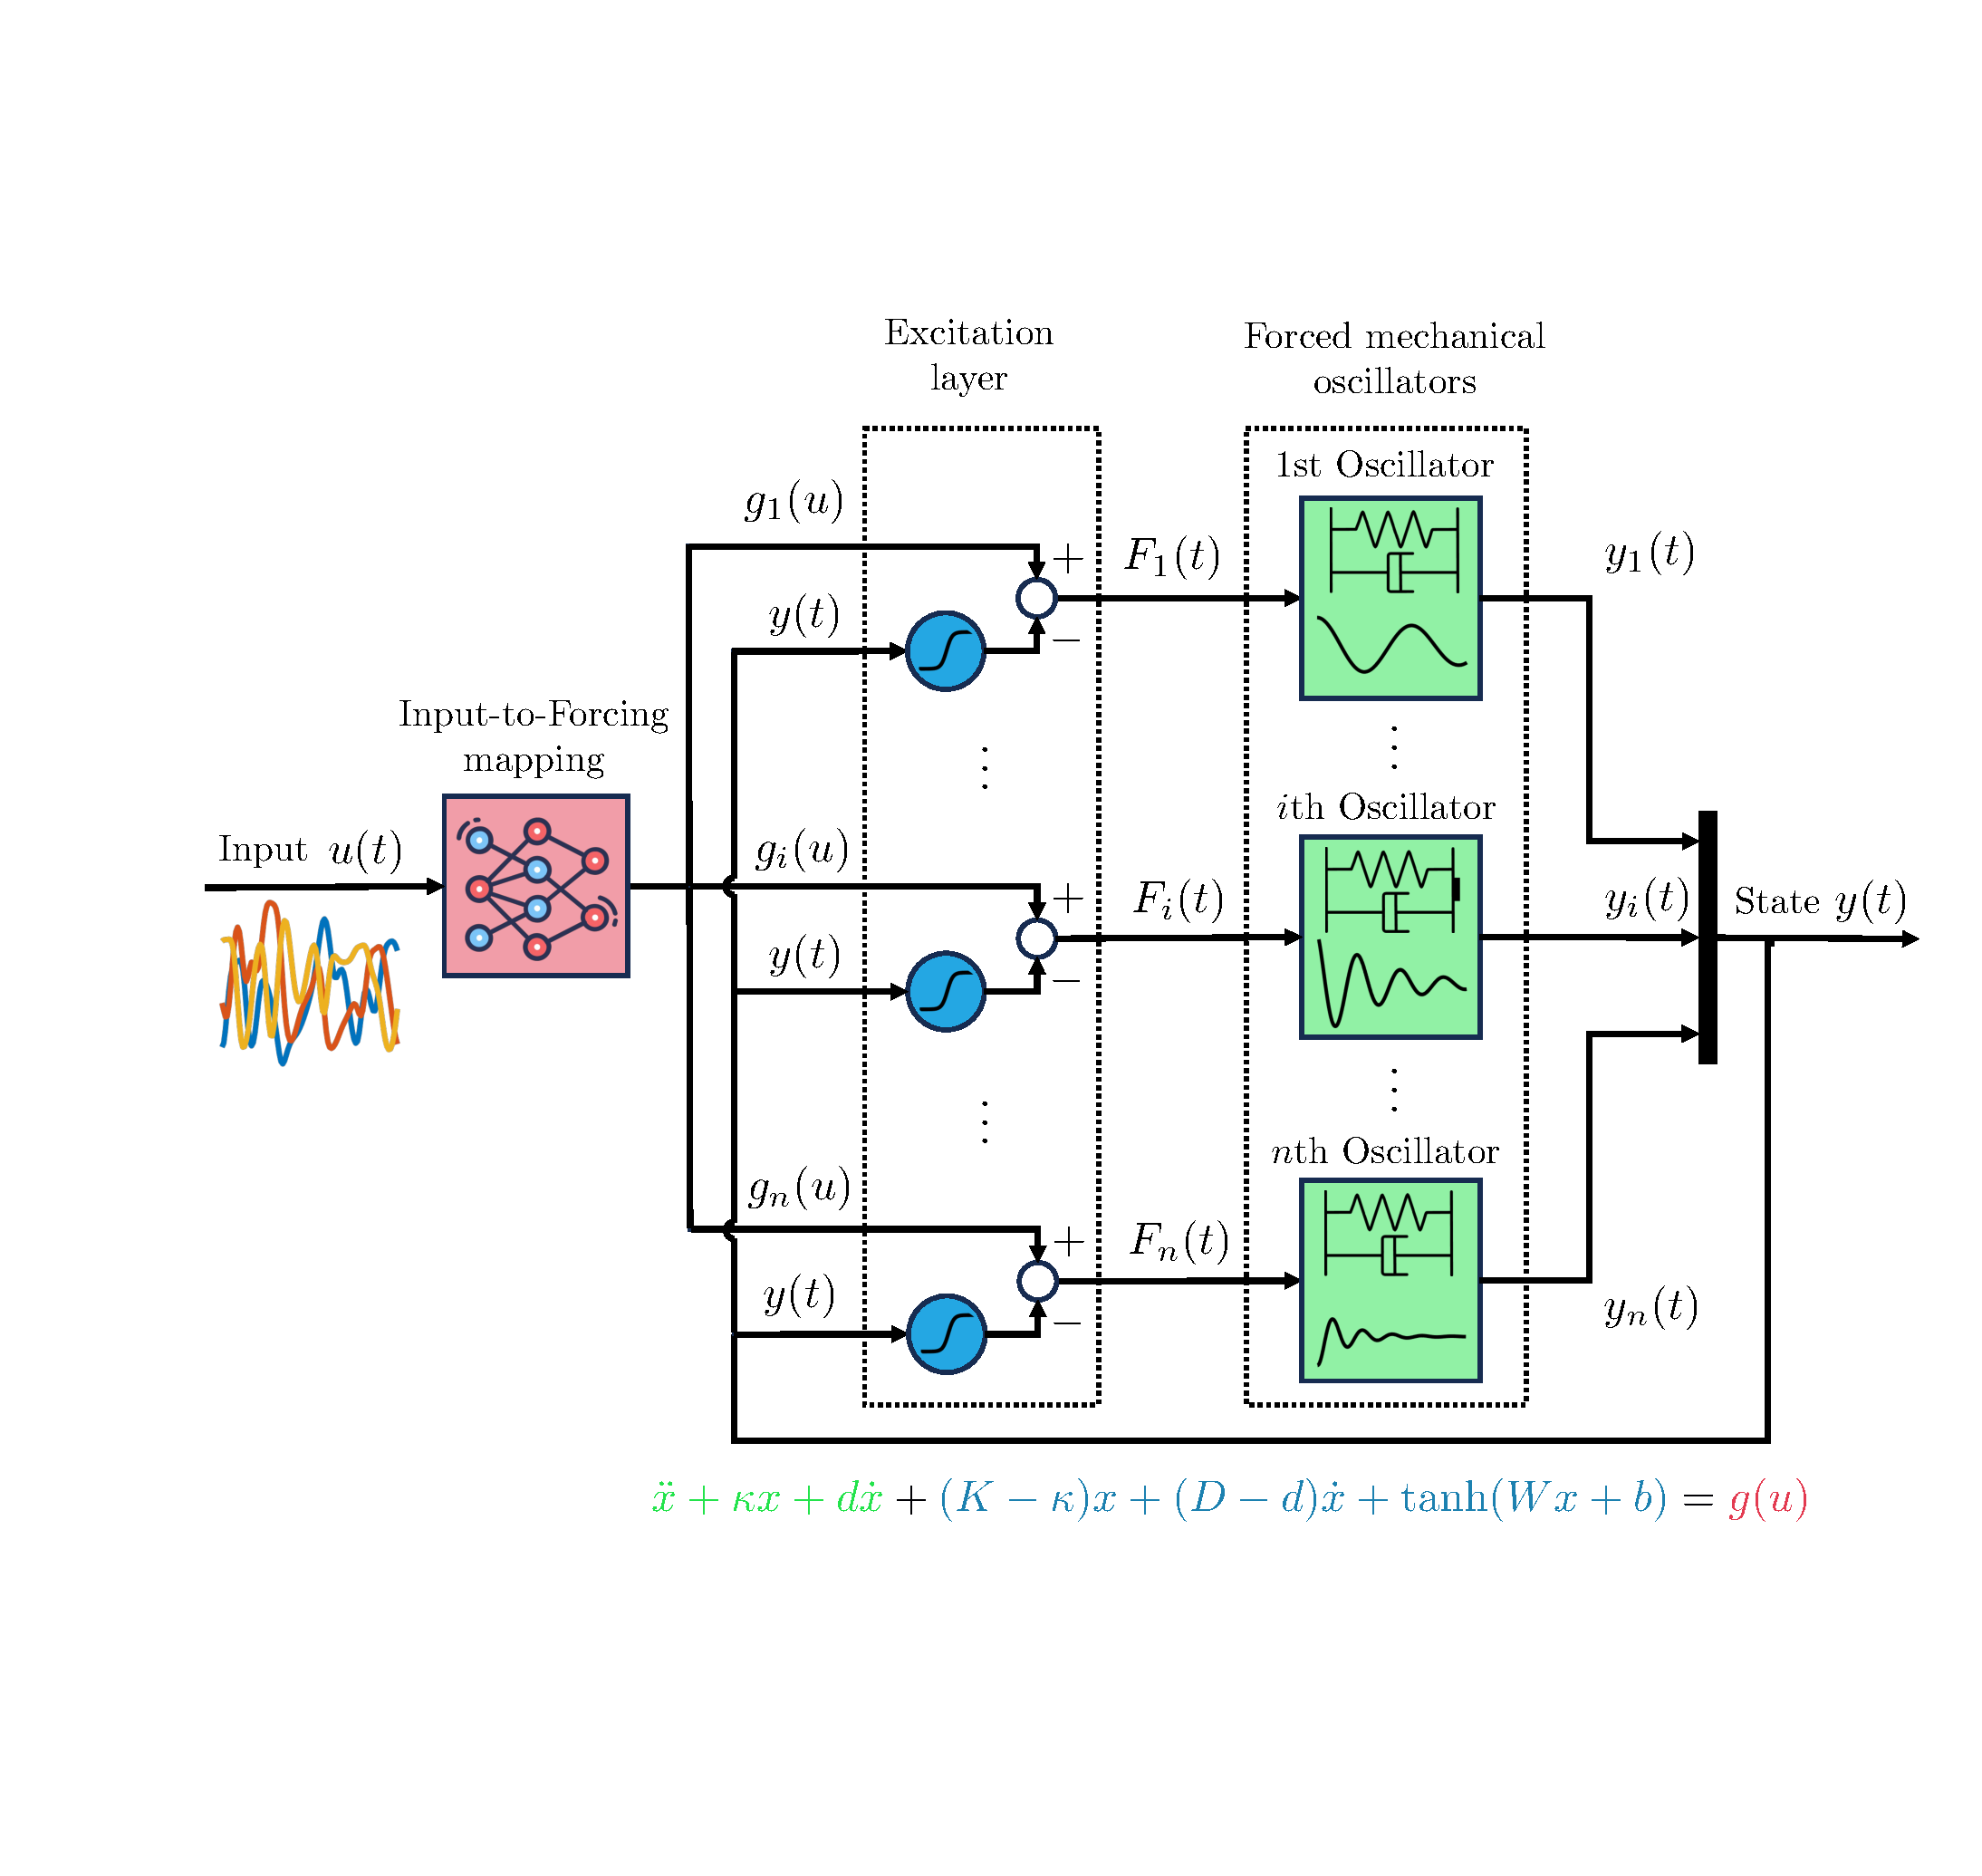
\includegraphics[width=0.45\columnwidth]{con/figures/con/blockdiagram_coupled_oscillator_network_v2_cropped.pdf}\label{fig:con:con}}
    \subfigure[Learning latent-space dynamics with CON]{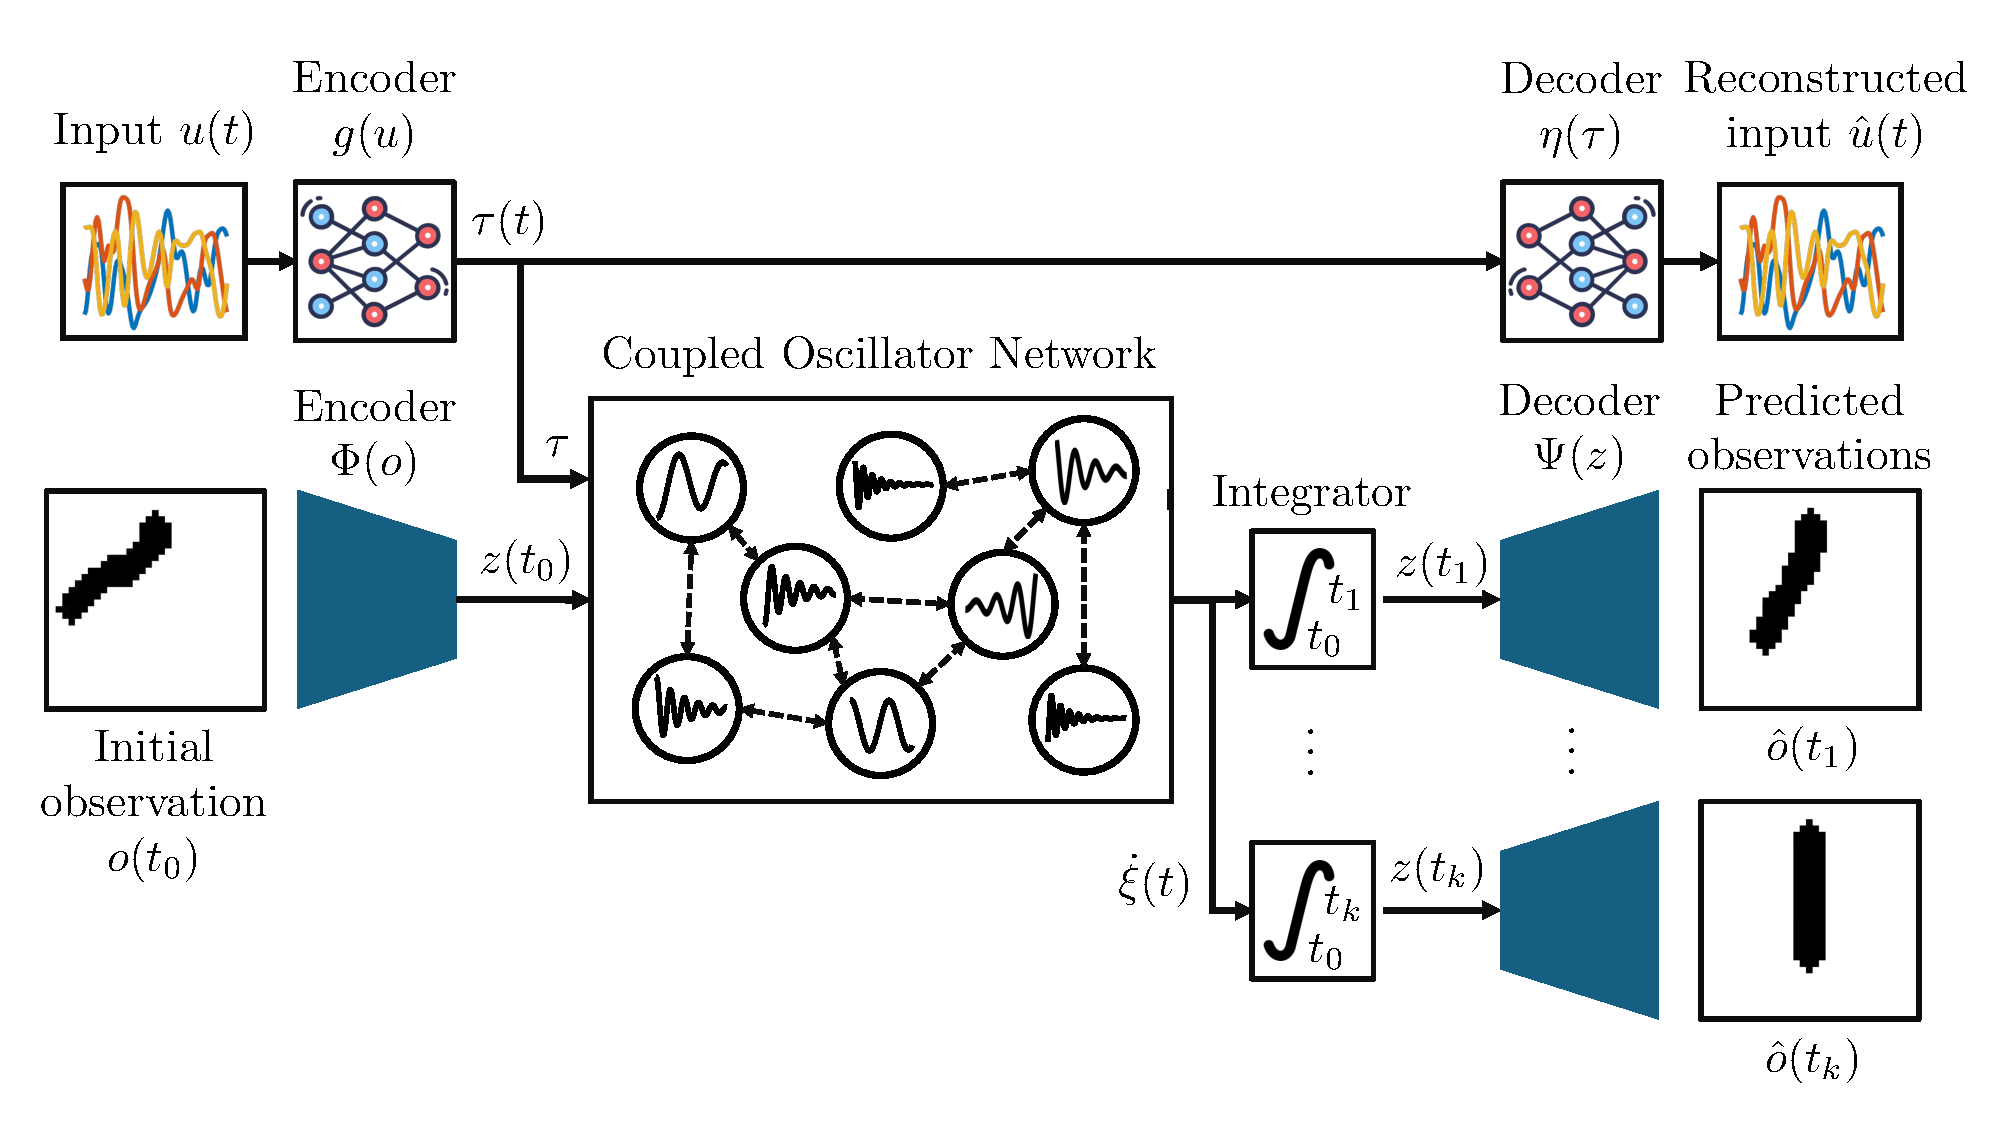
\includegraphics[width=0.53\columnwidth]{con/figures/autoencoder/blockdiagram_autoencoder_v1_cropped.pdf}\label{fig:con:blockdiagram_autoencoder}}
    \caption{\textbf{Panel (a)}: The proposed CON network consists of $n$ damped harmonic oscillators that are coupled through the neuron-like connection $\tanh(Wx+b)$ and the non-diagonal stiffness $K-k$ and damping coefficients $D-d$, respectively. The state of the network is captured by the positions $x(t)$ and velocities $\dot{x}(t)$ of the oscillators. The time-dependent input is mapped through the (possibly nonlinear) function $g(u)$ to a forcing $\tau$ acting on the oscillators. 
    \textbf{Panel (b):} Exploiting \glspl{CON} for learning latent dynamics from pixels: We encode the initial observation $o(t_0)$ and the input $u(t)$ into latent space where we leverage the \gls{CON} to predict future latent states. Finally, we decode both the latent-space torques $\tau(t)$ and the predicted latent states $z(t)$.
    }
\end{figure}

Subsequently, we derive an approximate closed-form solution, that is, in parameter regimes in which the linear, decoupled dynamics dominate transient, more accurate than numerical integrators with comparable computational requirements and which increases training speed by 2x with a small decrease in prediction accuracy.
Finally, as we can derive the system's potential energy, we can leverage potential shaping~\cite{bloch2001controlled, ortega2021pid} to derive a controller that combines an integral-saturated PID controller with a feedforward term compensating potential forces.
As the feedback acts on a well-shaped potential field, tuning the feedback gains becomes very simple and out-of-the-box, and the controller exhibits a faster response time and a \SI{26}{\percent} lower trajectory tracking \gls{RMSE} than a pure feedback controller based on a latent \gls{NODE}~\cite{chen2018neural} model.

The proposed methodology is particularly well-suited for learning the latent dynamics of mechanical systems with continuous dynamics, dissipation, and a single, attractive equilibrium point. Examples of such systems include many soft robots, deformable objects with dominant elastic behavior, Lagrangian systems immersed in a dominant potential field, or locally other mechanical systems such as robotic manipulators, legged robots, etc. For these systems, we can fully leverage the structural prior of the proposed latent dynamics, including the integrated stability guarantees. If the system is actuated, the learned dynamics can be subsequently exploited for model-based control, as demonstrated in Sec.~\ref{sec:con:latent_space_control}.

The code associated with this chapter is available on GitHub\footnote{\url{https://edu.nl/yu9vw}}.
Furthermore, we provide more details about the experimental setup and present additional results in Apx.~\ref{chp:apx:con}.

% In summary, our work makes the following contributions:
% \begin{itemize}
%     \item We propose a coupled oscillator network formulation with strong stability guarantees and a physical interpretation of its dynamics in terms of kinetic and potential energy that exhibits performance on par with the state-of-the-art, non-structured methods for learning dynamics in the tested situations.
%     \item We leverage for the first time oscillator networks for learning latent dynamics. This provides structure to the learned dynamics while preserving expressiveness.
%     \item The special characteristics of the network allow us to apply partial feedback linearization-based control techniques in a learned latent space.
%     \item An approximated closed-form solution for integrating the dynamics of the coupled oscillator network is provided, which is more accurate compared to numerical \gls{ODE} integrators with the same computational demand when the dynamics of underdamped, decoupled, and linear oscillators are dominant.
% \end{itemize}